
\section{Method}
\label{sec:method}

\par
The gears are to interface with the provided gear mounted on the test rig. A wrench would be attached to the one arm of the rig and turned to apply torque to the gears in the rig and subsequently to the arm applying the load to the load cell. The program interfacing with the Instrotech Model 4004 is set to start recording and the torque is applied until failure or the maximum load of 100 kg is applied to the load cell. The recorded results are exported as a .csv file and processed [\ref{im:testRig}].

\begin{figure}[H]
    \centering
        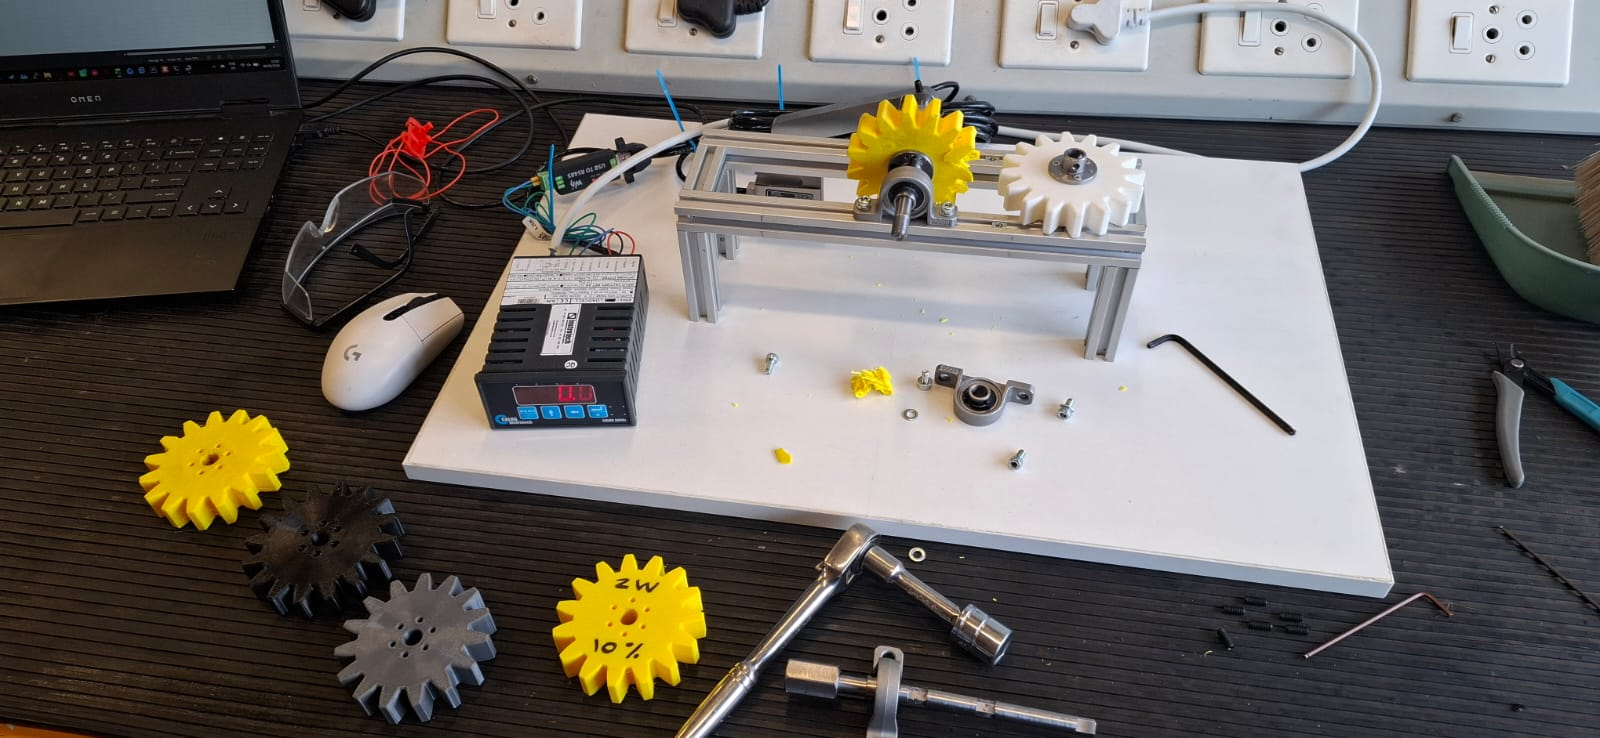
\includegraphics[width=0.75\textwidth]{img/im_testRig.jpeg}
        \caption{Rig Used to Test Gear Strength}
        \label{im:testRig}
\end{figure}

\par
To determine the results desired from the experiment, the following calculations and assumptions were made. A drum that has a height of 60mm and a diameter of 50mm was chosen. These were chosen so that the number of cable or rope can fit into only 1 wrap on the drum if the stroke is to be 1600mm if the rope were assumed to be 5mm in diameter. A mass of 30kg was assigned as the load of the drum at any one time to include the 20kg load with the equipment that might hang below it along with overhead. If the nominal speed of the motor is acheived at a speed of 1360 rpm with power of 0.18kW, then the gears need to withstand approximately 11,036Nm [\ref{eq:drum_torque}] if one is to withstand the maximum torque of the drum at any one time. It is unlikely that this top speed will be achieved by the motor due to the VFD limitations so these specifications will be prone to change [\ref{app:A_excel}].

\[
\tau_{\mathrm{Drum}} = \mathrm{Load} \times 9.81 \times \frac{\varnothing_{\mathrm{Drum}}}{2 \times 1000} \times K_{\mathrm{Serving\ Factor}}
\]

\par
Using the maximum load from the results, the torque applied to the gear can be determined and compared to the required torque. The test rig arm pressing onto the load cell is 100mm long[\ref{eq:rig_torque}].
\[
    \tau = F \times d
\]
